\section{Закон электромагнитной индукции Фарадея в интегральной и
дифференциальной формах.}

\begin{minipage}[c]{0.4\textwidth} % Левая часть: изображение
    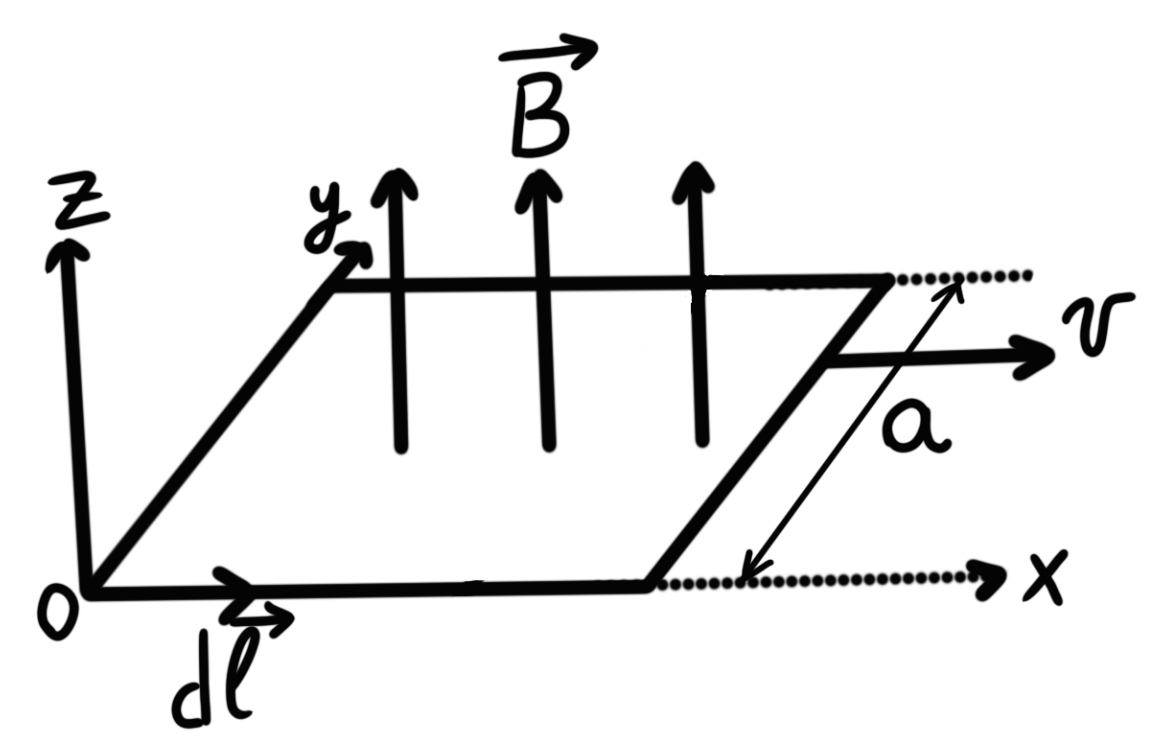
\includegraphics[width=\textwidth]{im/85.png}% Ваше изображение
\end{minipage}%
\hfill
\begin{minipage}[c]{0.6\textwidth} % Правая часть: текст
    \begin{gather*}
        \varepsilon=\oint \vec{E}_{\text{сторонняя}}d\vec{l}=\oint \frac{\vec{F}_{\text{ст}}}{q}d\vec{l}= \\
        =\frac{1}{c}\oint [\vec{v}\times \vec{B}]d\vec{l}=-\frac{1}{c}vaB   
    \end{gather*}
\end{minipage}

\[
\frac{d\Phi}{dt}=\frac{d}{dt}(a \times B)=aB \frac{dx}{dt}=aBv   
\]

\[
\varepsilon=-\frac{1}{c}vaB=-\frac{1}{c}\frac{d\Phi}{dt}   
\]

\begin{minipage}[c]{0.4\textwidth} % Левая часть: изображение
    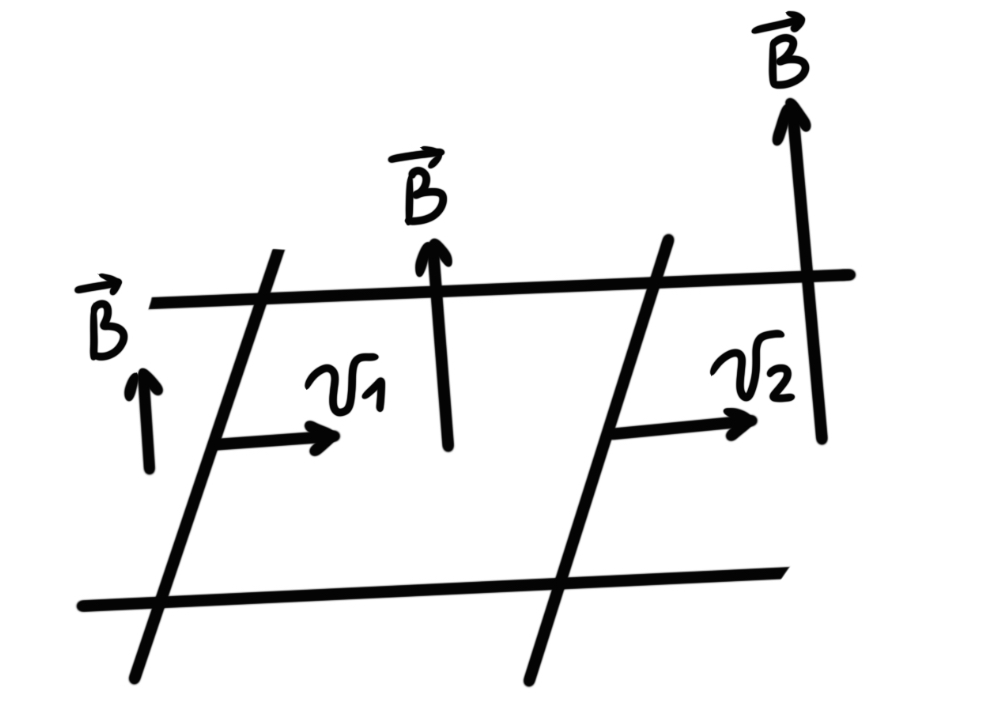
\includegraphics[width=\textwidth]{im/86.png}% Ваше изображение
\end{minipage}%
\hfill
\begin{minipage}[c]{0.6\textwidth} % Правая часть: текст
    \begin{gather*}
        \varepsilon=-\frac{1}{c}v_2B_2a-\frac{1}{c}v_1B_1a \\
        \frac{d\Phi}{dt}=aB_2v_2-aB_1v_1 \\
        \Rightarrow \varepsilon=-\frac{1}{c}\frac{d\Phi}{dt}   
    \end{gather*}
\end{minipage}

Расмтрим \( \varepsilon \) для прозвольного контура: 

\begin{minipage}[c]{0.4\textwidth} % Левая часть: изображение
    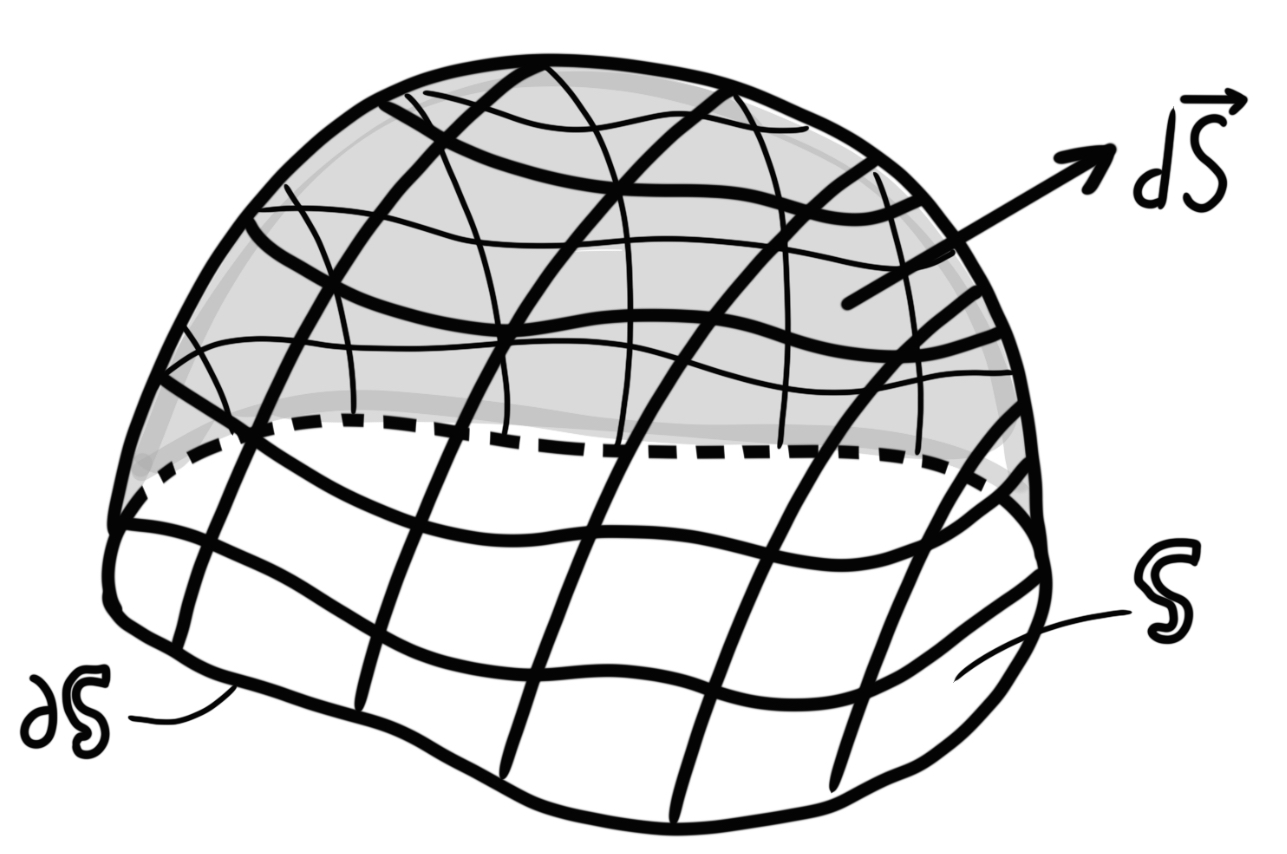
\includegraphics[width=\textwidth]{im/87.png}% Ваше изображение
\end{minipage}%
\hfill
\begin{minipage}[c]{0.6\textwidth} % Правая часть: текст
    \begin{gather*}
        \Phi=\underset{\mathbb{S} }{\oiint}\vec{B}d\vec{S} \qquad \varepsilon=\underset{\partial \mathbb{S} }{\oint}\vec{E}d\vec{l}
    \end{gather*}
\end{minipage}

